\documentclass[11pt]{article}
\usepackage{graphicx}
\usepackage{hyperref}
\usepackage{natbib}

\setlength{\textwidth}{6.5in}
\setlength{\headheight}{0in}
\setlength{\textheight}{8.0in}
\setlength{\hoffset}{0in}
\setlength{\voffset}{0in}
\setlength{\oddsidemargin}{0in}
\setlength{\evensidemargin}{0in}

\title{Computational Physics: Problem Set 8}

\author{Zifeng Li}
\begin{document}
\maketitle

\section{Questions}

\subsection{Question 1}
The resulted graphs are shown below. I use scipy.fft to perform Fourier Transform.
\begin{figure}[b!]
\centering
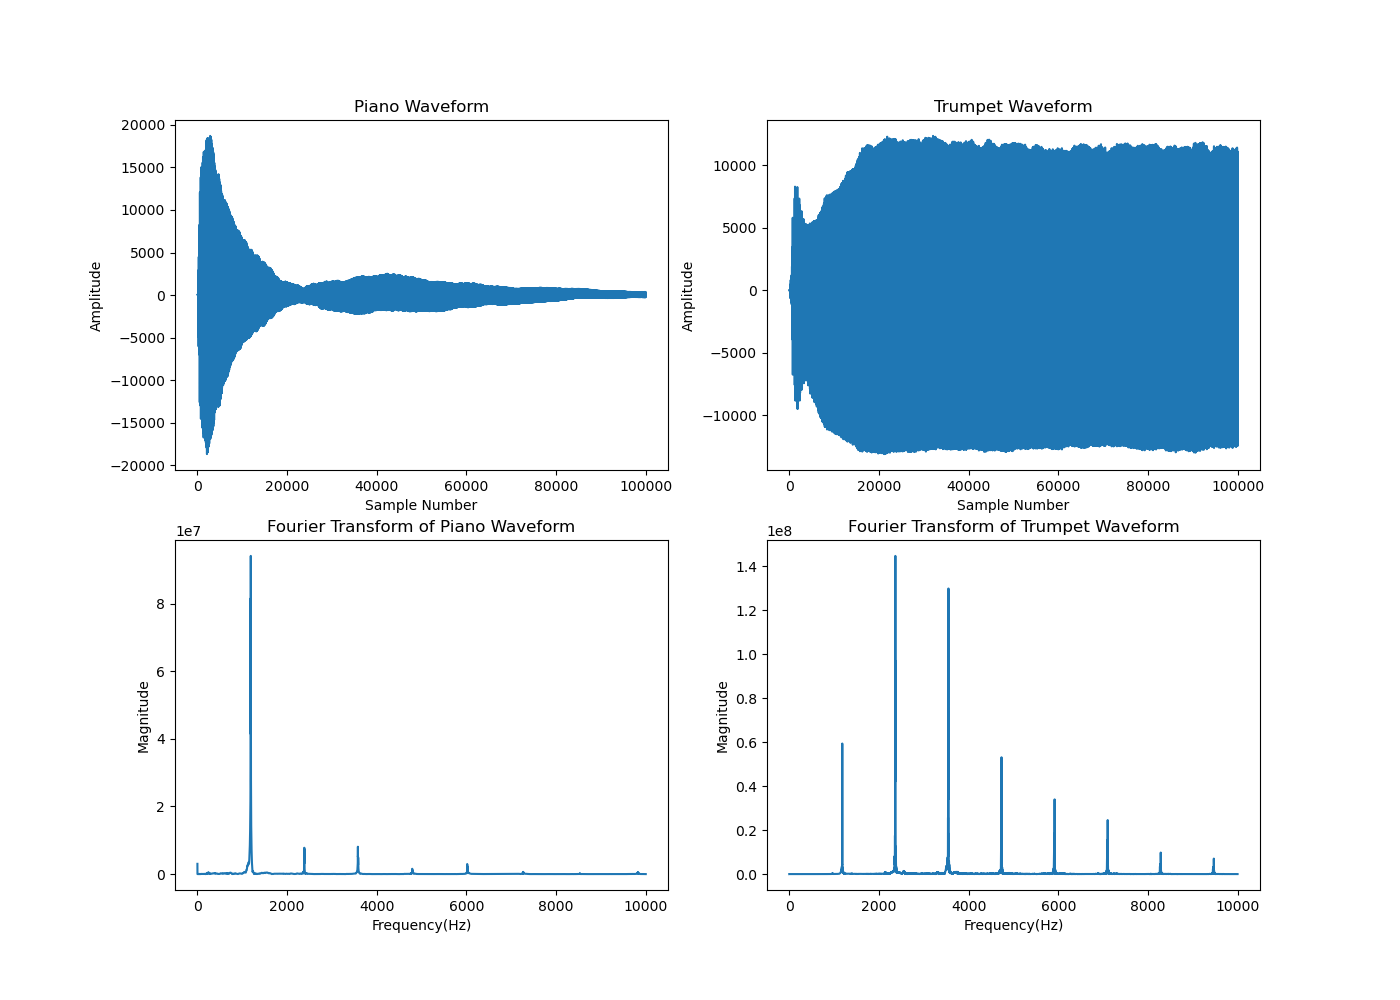
\includegraphics[width=0.95\textwidth]{Instrument Waveform and Their Fourier Transform.png}
\end{figure}



\subsection{Question 2}
The two graphs generated here represent Lorenz equations in a plot of y against
time and a plot of z against x, which is also known as the attractor.
The motion appears to be unpredictable and sensitive to initial conditions, which
means that even small changes in the initial state can lead to significantly different outcomes.

\begin{figure}[b!]
\centering
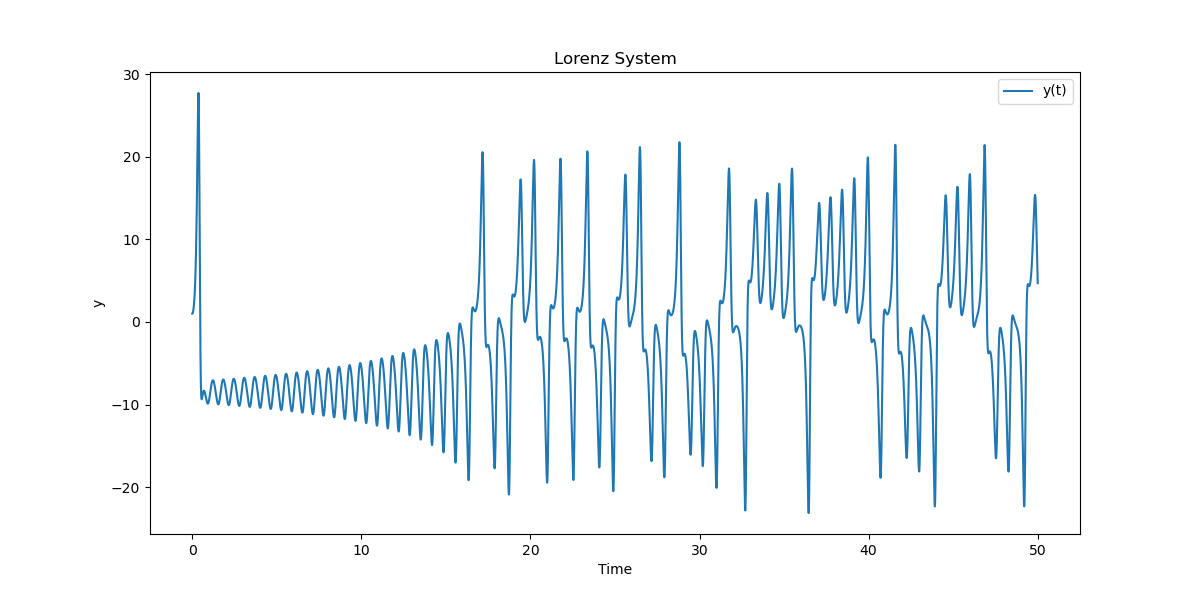
\includegraphics[width=0.95\textwidth]{Lorenz System.png}
\end{figure}

\begin{figure}[b!]
\centering
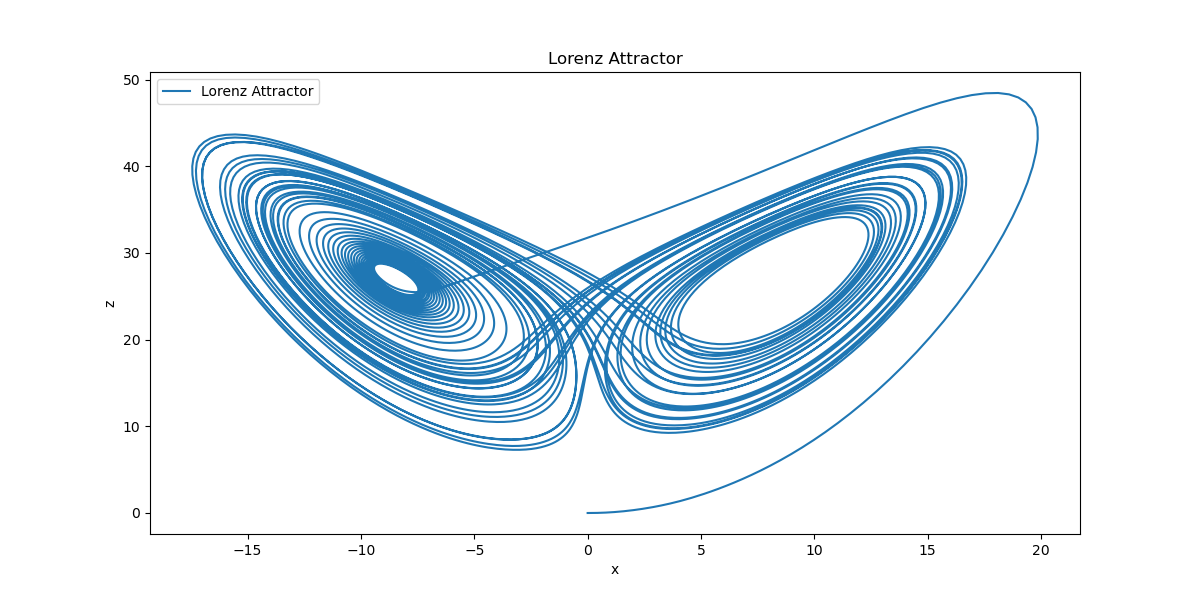
\includegraphics[width=0.95\textwidth]{Lorenz Attractor.png}
\end{figure}





\end{document}
